\documentclass[11pt]{article}

% %%%%%%%%%%%%%%%%%%%%%%%%%%%%%%%%%%%%%%%%%%%%%%%%%%%%%%%%%%%%%%%%%%%%%%%%%%%%%%
% %                                 PACKAGES                                   %
% %%%%%%%%%%%%%%%%%%%%%%%%%%%%%%%%%%%%%%%%%%%%%%%%%%%%%%%%%%%%%%%%%%%%%%%%%%%%%%

% Identify input as UTG-8 format
\usepackage[utf8]{inputenc}

% Style Helvet
\usepackage{setspace}
 \singlespacing
\usepackage[scaled]{helvet}
 \renewcommand\familydefault{\sfdefault}
\usepackage[T1]{fontenc}

% Equations
\usepackage{amsmath}

% Code
\usepackage{listings}
\usepackage[cache=false]{minted}
 \listfiles

% Item Enumeration
\usepackage{enumitem}
% Easy List
\usepackage[ampersand]{easylist}

% Tables
\usepackage{booktabs}
\usepackage{longtable}

% Margins
\usepackage{geometry}
 \geometry{
  a4paper,
  left=25mm,
  top=25mm,
  right=25mm,
  left=25mm
 }

% Images
\usepackage{float}
\usepackage{graphicx}
\usepackage{subcaption}

% Positions and locations
\usepackage{float}

% References
\usepackage{hyperref}

% %%%%%%%%%%%%%%%%%%%%%%%%%%%%%%%%%%%%%%%%%%%%%%%%%%%%%%%%%%%%%%%%%%%%%%%%%%%%%%
% %                                  TITLE                                     %
% %%%%%%%%%%%%%%%%%%%%%%%%%%%%%%%%%%%%%%%%%%%%%%%%%%%%%%%%%%%%%%%%%%%%%%%%%%%%%%

\title{Courseworkv 1: Experimental Comparison of k-NN and Linear Classification
on the Iris data-set}

\author{
Acereda García, Pablo\\
19043879}

% %%%%%%%%%%%%%%%%%%%%%%%%%%%%%%%%%%%%%%%%%%%%%%%%%%%%%%%%%%%%%%%%%%%%%%%%%%%%%%
% %                               DOCUMENT                                     %
% %%%%%%%%%%%%%%%%%%%%%%%%%%%%%%%%%%%%%%%%%%%%%%%%%%%%%%%%%%%%%%%%%%%%%%%%%%%%%%

\begin{document}

% Title
\maketitle

% This page has been left blank intentionally
\newpage
\vspace*{\fill}
 \begin{center}
This page has been left blank intentionally
 \end{center}
\vspace*{\fill}
\newpage

% Table of contents
\tableofcontents

\newpage

%                            %%%%%%%%%%%%%%
%                             INTRODUCTION
%                            %%%%%%%%%%%%%%
\section{Introduction - Machine Learning and Classification Problems}

Machine learning, is a field of study which is on the search for predictions
towards a certain given input. But the input does not automatically transform
into the right answer, by divine intervention. But as a science worthy of its
name, it relies on mathematical models which are the result of using statistical
models and artificial intelligence (AI).

The process of transformation of a certain input, or training data; to the
desired output, is known as classification problem.

In this process, there can be identified three main categories: 
\textit{supervised learning}, \textit{unsupervised learning} and
\textit{reinforcement learning}.

\begin{description}
 
 \item [Supervised Learning] A problem gets this name when the input goes with
  its expected output, so the function obtained to classify new inputs comes
  from labeled training data.
 
 \item [Unsupervised Learning] In this case, no data is labeled. On the 
  contrary, unsupervised search helps finding clusters in data (and therefore 
  labelling them) or to find correlation in sets of possibly correlated 
  observations.

 \item [Reinforcement Learning] The objective of these algorithms is to maximize
  some notion of cumulative reward, given a certain enviroment and deciding
  which actions should take a software agent\footnote{''Computer program that
  acts for a user or other program.''}.

\end{description}

The scope of this assignment is not to delve into unsupervised learning; nor is
to go into detail about reinforcement learning (which has not even been 
mentioned in the lectures so far).

In the following sections of the project, it is going to be discussed about the
dataset used; give a description of the algorithms exploited; and comment how
those models are applied to the given dataset.

%                                 DATASET
%                                =========
\subsection{Dataset - Iris Dataset}

Also known as \textit{Iris flower data set} or \textit{Fisher's Iris data set}
(name given after Ronald Fishers, who used the dataset in his publication in 
1936); is a dataset formed by three flowers from the same species: \textbf{Iris 
flowers}.

According to the original paper, \textit{``All three species were collected in
the Gaspé Peninsula, from the same pasture, picked on the same day and measured
at the same time by the same person with the same apparatus''}.

The three species that the original paper talks about are:

\begin{easylist}[itemize]
 
  & Iris Versicolor
  & Iris Setosa
  & Iris Virginica

\end{easylist}

\begin{figure}[H]
 \centering
 \begin{subfigure}{0.32\textwidth}
  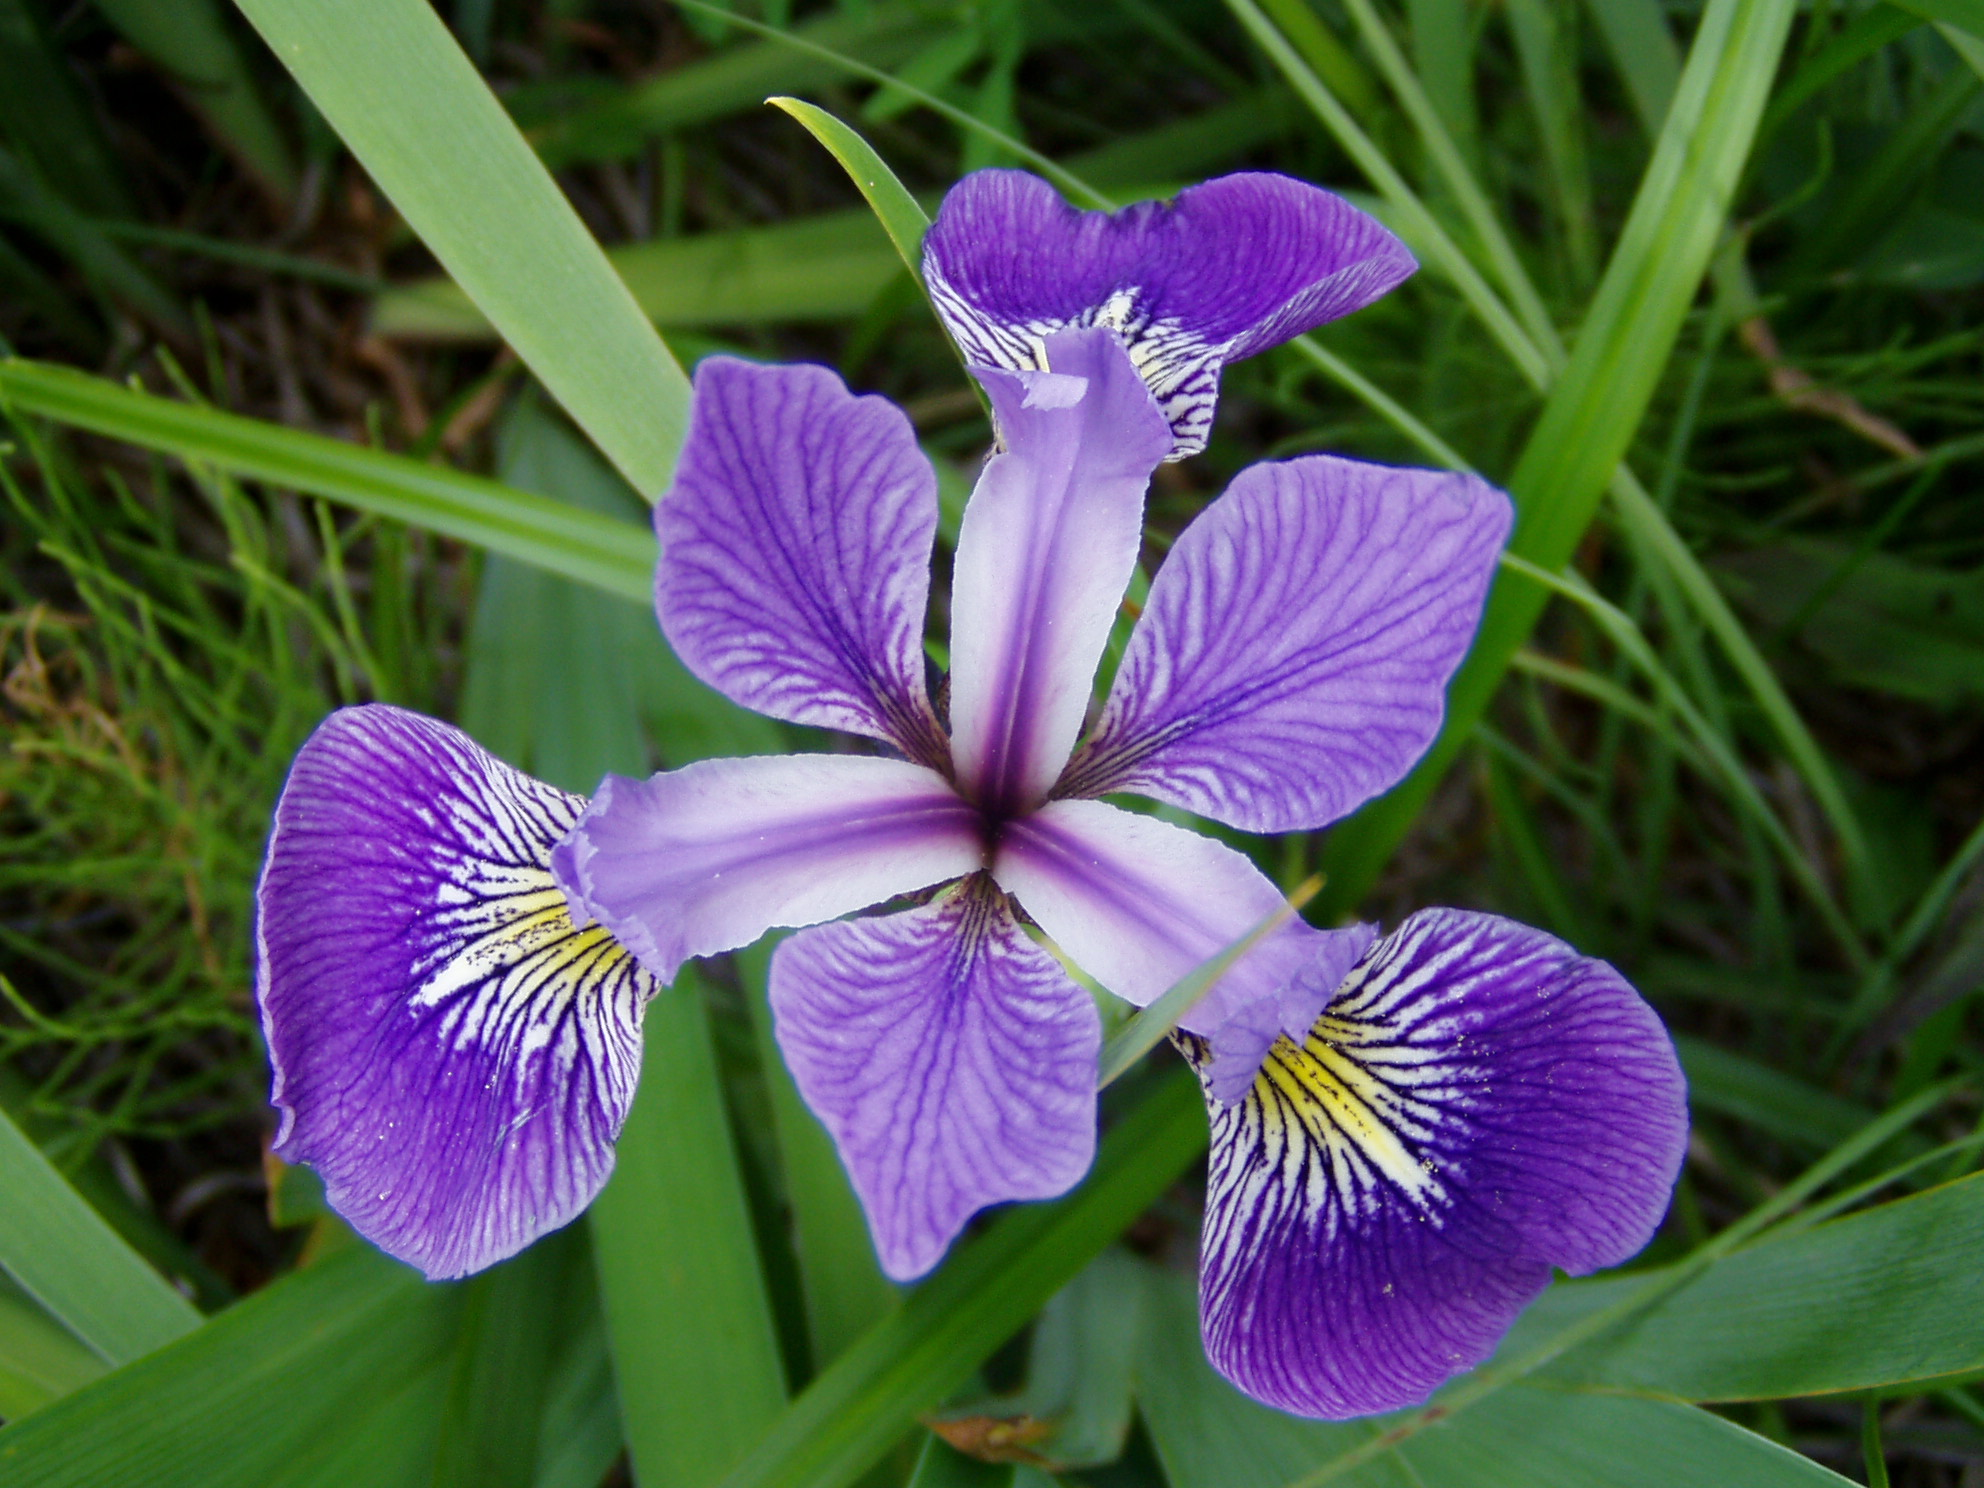
\includegraphics[width=0.9\linewidth]{../images/iris_versicolor.jpg}
  \caption{Iris Versicolor}
 \end{subfigure}
 \begin{subfigure}{0.32\textwidth}
  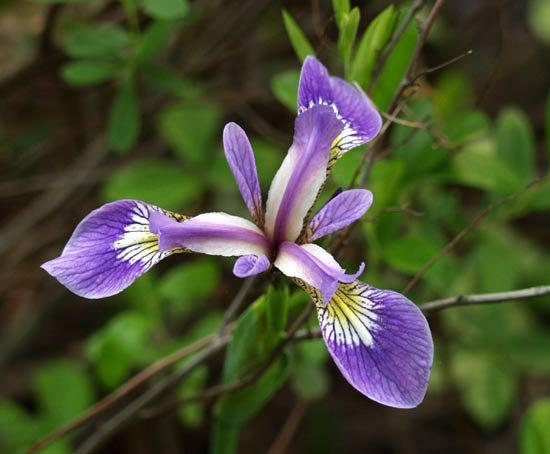
\includegraphics[width=0.9\linewidth]{../images/iris_setosa.jpg}
  \caption{Iris Setosa}
 \end{subfigure}
 \begin{subfigure}{0.32\textwidth}
  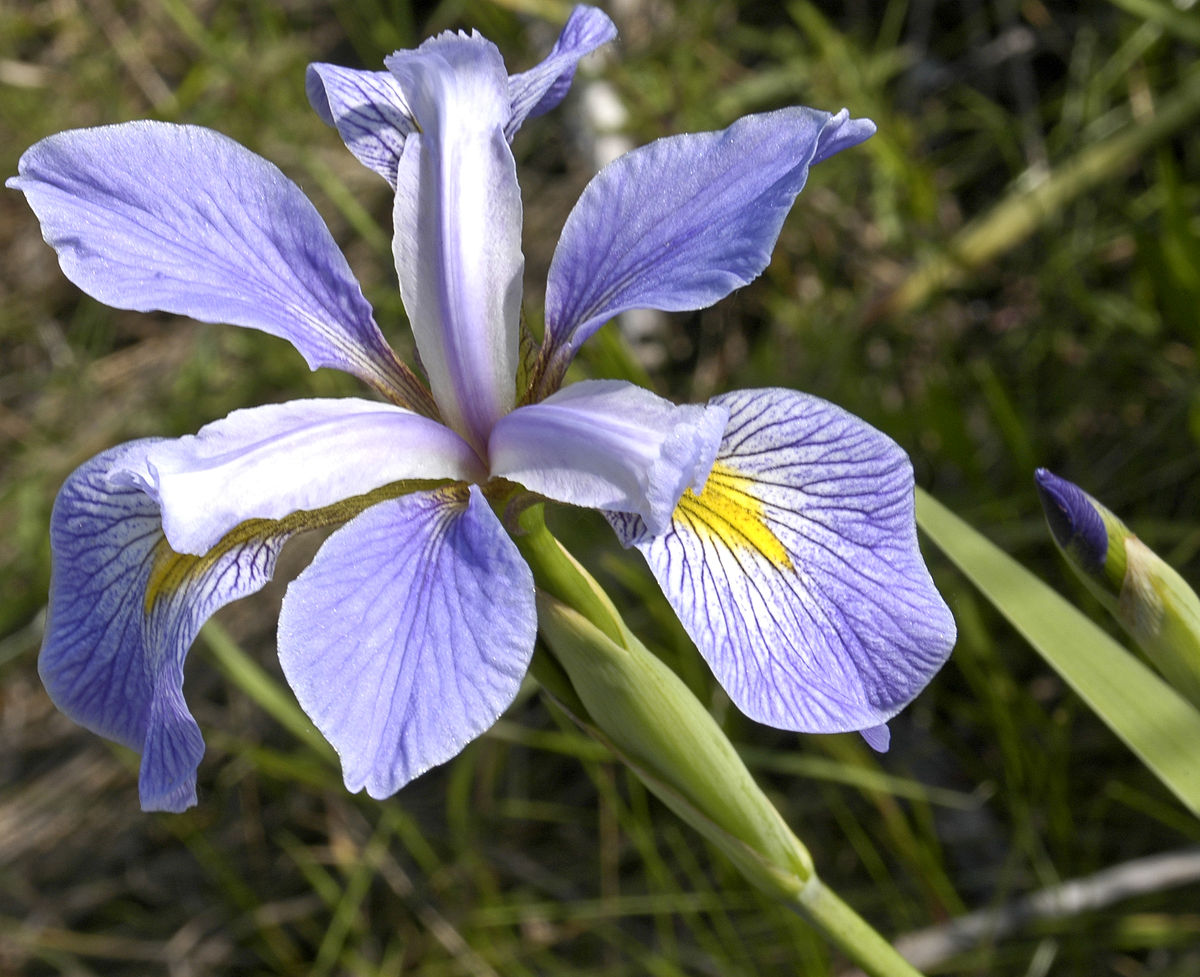
\includegraphics[width=0.9\linewidth]{../images/iris_virginica.jpg}
  \caption{Iris Viginica}
 \end{subfigure}

\end{figure}

There were measured the characteristics of 50 flowers from each particular
specie; taking into account the length and the width from sepals and petals. The
unit of measure used was centimiters (cm).

\begin{figure}[h]
 \centering
 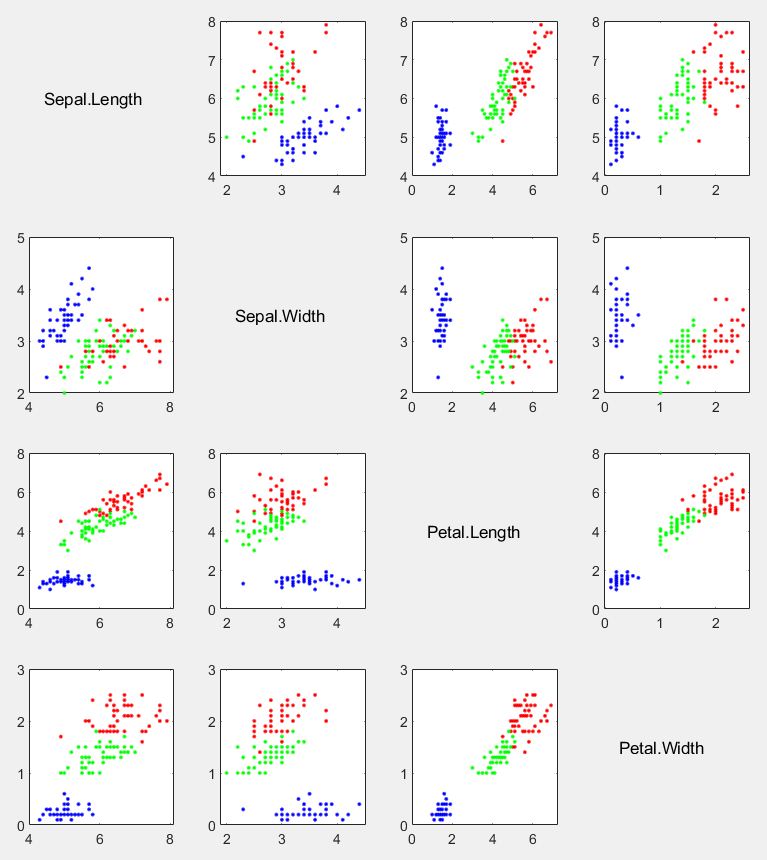
\includegraphics[width=0.65\textwidth, height=10cm]
                 {../images/characteristics.png}
 \caption{Attributes Relation.}
\end{figure}

In this specific project, the Iris Dataset has been used to train and test kNN
and linear classification, randomly ordering the samples to later apply
cross-valitadion method k-fold.

%                                 MODELS
%                                ========
\subsection{Models - kNN and Linear Classification}

%                            ===== KNN =====
\subsubsection{K-Nearest-Neightbors}

To classify a new input, by checking which are the closest neightbors; that is
the scope this classification method uses. It is possible to understand how it
works at a glance, when the model is trained by labeled data, it can predict the
class/specie/category of the sample just by computing the k-nearest neightbours;
using the \textit{euclidean distance}.

For two dimensions, the formula goes as follows:

\begin{equation}
 \centering
 \sqrt{(x_1 - x_2)^2 + (y_1 - y_2)^2}
\end{equation}

When used in MATLAB, it allows multiple options.

\begin{minted}{matlab}
 Mdl = fitcknn(Tbl, ResponseVarName/formula/Y)
 Mdl = fitcknn(X, Y)
 Mdl = fitcknn(__, Name, Value)
\end{minted}

To ease things, \textit{Tbl and X} are attributes from the samples of data 
used to train the model; \textit{ResponseVarName and Y} are the desired output
for the clusters of samples.

\textit{formula} intends to give an equation on how \textit{Y} depends on the
predictor variables.

A very important argument, or list of arguments, which can be specified after
any of the aforementioned variables is the \textit{Name-Value} Pair Arguments.
They allow to edit properties like what breaks ties in case several samples have
the same properties; the value for k (how many neightbors are selected to decide
the specie), \ldots

%                     ===== LINEAR CLASSIFICATION =====
\subsubsection{Linear Classification}

There are actually 2 models which create a linear classification:
\textit{fitclinear} and \textit{fitcecoc}. As the first of the does not allow
multiclass models such the needed for Iris Dataset, that is the one to be
described in this section.

In any case, they both use linear equations to ``separate'' the points from each
specie. If a given sample is in the area of a certain specie, the model decides
it belongs to that same specie.

\begin{equation}
 \centering
 y = a * bx
\end{equation}

\begin{minted}{matlab}
 Mdl = fitcecoc(Tbl, ResponseVarName/formula/Y)
 Mdl = fitcecoc(X, Y)
 Mdl = fitcecoc(__, Name, Value)

 [Mdl, HyperparameterOptimizationResults] = fitcecoc(__)
\end{minted}

At first sight it can be seen that both linear and kNN classification have very
similar parameters.

The diference can be found for eample in the pair of arguments
\textit{Name-Value}. Can modify the behaviour of the binary learners, design
partitions, \ldots

There is also one more variable, \textit{HyperparameterOptimizationResults},
which is the description of the cross-validation optimization of
hyperparameters. It is not going to be used, as the cross-validation is to be
implemented manually.

%                                APPLICATION
%                               =============
\subsection{Application - Models to Dataset}

All these theory is very accurate, and also compelling but, how is this going to
help with the Iris Dataset? Fairly simple, by creating different models that
should be able to predict the specie of new inputs of data.

With kNN, the more neightbors that are from the same specie, the more chances
that input has to be from that specie. Varying values for k might also be
helpful when it comes to accuracy.

On the other hand, linear classification uses multiclass linear equations to
predict if the given new sample is from one specie or not. In this case, no
parameters have been changed.

%                           %%%%%%%%%%%%%%%%%%%
%                            EXPERIMENTAL WORK
%                           %%%%%%%%%%%%%%%%%%%
\section{Experimental Work}

The aforementioned models have been implemented in MATLAB, in addition to other
statistical methods and algorithms in order to predict new samples from the
species \textit{Iris Versicolor}, \textit{Iris Setosa} and \textit{Iris
Virginica}.

To make it more bearable, the structure of the program could be simplified as
follows:

\begin{easylist}[enumerate]
 
  & K-fold implementation. Henceforth, Data must me splitted in k same-sized
  pieces. 
  
  & Model generation on training data from \textit{Iris Dataset}, previously
  separated by k-fold: \textbf{fitcknn} and \textbf{fitcecoc}.

  & Test models by predicting labels from testing data.

  & Compute error based on the predicted labels and their actual values.

  & Select least error model, as the average of the k-folding implementation.

  & Data visualization.

\end{easylist}

%                              CROSSVALIDATION
%                             =================
\subsection{Crossvalidation - K-fold}

As it has been mention before, it has been implemented crossvalidation using
k-folding. It works by splitting data in k same-sized parts, and iterating
through them, so every chunck of data is being used for training and for
testing.

\begin{figure}[h]
 \centering
 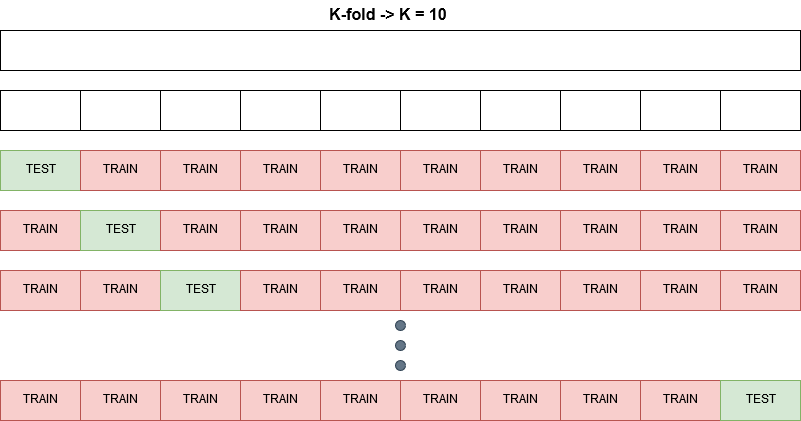
\includegraphics[width=0.75\textwidth]{../diagrams/kfold.png}
 \caption{K-fold crossvalidation.}
\end{figure}

\subsection{Modeling and Testing - fitcknn and fitcecoc}

The complexity of this procedure is not inherently very high; once data has been
separated into chunks from the same size, it is just needed to specify certain
parameters at most (\hyperref[mdls]{\ref{mdls}}).

It is not needed any forward step to obtain and test the models.

\subsection{Error - Cost Function}

The implementation chosen for this problem is not other than the Mean Error
(ME - \hyperref[me]{\ref{me}}).

\begin{equation}
 \centering
 \frac{1}{N} \sum_{i=1}^{N} {I(a, b)} \label{me}

 \begin{cases}
  I(a, b) = 1, if a \neq b\\
  I(a, b) = 0, if a = b
 \end{cases}
\end{equation}

The usage of any other studied error equation would be absurd. For example,
taking the Mean Squared Error (MSE - \hyperref[mse]{\ref{mse}}):

\begin{equation}
 \frac{1}{N} \sum_{i=1}^{N} {I(a, b)^2} \label{mse}
\end{equation}

To square something which has a binary value, 0 or 1\footnote{Should be taken
into accout that the predicted label for the sample data can only be right or
wrong}, would actually result in the same value. 

Same happens with the Root Mean Squared Error (RMSE - 
\hyperref[rmse]{\ref{rmse}}), only in this case it would be with the square root 
of the same result that would be obtained with ME (Equation 
\hyperref[me]{\ref{me}}) but in this case proportional to the square root. 
Which, at least for the scope of this project is not really necessary.

\begin{equation}
 \sqrt{\frac{1}{N} \sum_{i=1}^{N} {I(a, b)^2}} \label{rmse}
\end{equation}

There is another function already implemented in MATLAB called 
\textbf{resubLoss}, but uses weights in the model and other parameters that are
not available, albeit it is more accurate, it cannot be implemented.

\section{Conclusion}

In brief, it has been used two different classification models, changing
individual parameters; also, the implementation of k-fold crossvalidation which
lead to the best overall trained model for both linear and kNN classifications.

But the results seem to conclude that the dataset is not large enough, as the
models most of the models give a 100\% of accuracy, which suggest that for
values of k, in k-fold crossvalidation, over 10 the testing data is not large 
enough. On the other hand, if in k-fold crossvalidation, if k is reduced so that 
testing data has a larger number of samples, the training data is not enough to 
train a good model.

Despite that fact, kNN perceives a lost in accuracy when k becomes too large
(it has been tested with values of k = 50 or k = 100). Albeit, once again due to
the number of samples being too small, changing values of k when k < 10 does not
really change the classification of the tested samples. According to
documentation found from kNN classification, it can be used the method known as
\textit{Elbow Method}, where the optimal value for k is found by iterating
through different k values, and using kfold crossvalidation (where 5 <= k <=
10). The conclusion remanins the same, there are not enough samples to perform
such a method with valid results.

Also, other aspect that should be taken into account is the resources
consumption of kNN algorith, which as sustantially higher than Linear
Classification, so available resources could also be the key point to decide on 
the algorithm to use. Not to mention, kNN is more time consuming that Linear
Classification. 

I would personally recommend Linear Classification, the error obtained is not
very different from kNN, but it consumes less resources.

\newpage

\section*{Appendix: Code}

As any respected MATLAB implementation, first of all is needed to have a clean
enviroment:

\begin{minted}{matlab}
% clear variables
% close opened windows
% clean the comand windows
%-------------------------------------------------------------------------%
clear variables;
close all;
clc;
%-------------------------------------------------------------------------%
\end{minted}

Now it is turn to load the data, and order it randomly so that later it is
easier to perform the k-fold crossvalidation.

\begin{minted}{matlab}
% %%%%%%%%%%%%%%%%%%%%%%%%%%%%%%%%%%%%%%%%%%%%%%%%%%%%%%%%%%%%%%%%%%%%%%%%%

% COURSEWORK 1: EXPERIMENTAL COMPARISON OF K-NN AND LINEAR CLASSIFICATION
% ON THE IRIS DATA-SET
% AUTHOR: PABLO ACEREDA

% %%%%%%%%%%%%%%%%%%%%%%%%%%%%%%%%%%%%%%%%%%%%%%%%%%%%%%%%%%%%%%%%%%%%%%%%%

%                              LOAD DATA
%                             ===========
load fisheriris
    
%                                DATA 
%                               ======
    
% Want to order samples randomly to apply cross-validation
P = randperm(length(species));

% Data from flower (all in cm):
% { Sepal length | Sepal width | Petal length | Petal width }
X = meas(P, :);

% Class label:
% - Setosa
% - Versicolor
% - Virginica
Y = species(P);
\end{minted}

Once the data is obtained, it might be a good idea to ask the user on the size
of the chunks of data. It has also been implemented a log file from which all
operations will be recovered post-execution.

\begin{minted}{matlab}
%                     DATA PARTITIONING INFORMATION
%                    ===============================

kDiv = input(['How many divisions do you want in the sample data ', ...
              '(more that one divisions: (k > 1)?\n']);
N    = length(species);
jump = ceil(N / kDiv);
%                          LOG FILE CREATION
%                         ===================

% File name
filename = 'experiments.log';
% Moves path to file's path
cd(fileparts(mfilename('fullpath')));

% Creates file in case it does not existe
edit(filename);
% Open file 
logFile = fopen(filename, 'w');

% Writes in log file
fprintf(logFile,                                           ...
        ['INFO: ',                                         ...
         '==== NEW EXPERIMENT ====\n',                     ...
         'INFO: ',                                         ...
         'Data is going to be divided into %i pieces.\n'], ...
        kDiv);
\end{minted}

Some other variables and data is needed along the execution of the program. It
is a good practice to initialize the values and the format before they are used.

\begin{minted}{matlab}
% Valid number of divisions
if kDiv < N
    
    % Write into log
    fprintf(logFile,                             ...
            ['INFO: ',                           ...
             'The value for k is valid ',        ...
             '(k[%i] < number of samples[%i]) ', ...
             '-> VALID.\n'],                     ...
            kDiv,                                ...
            N);
    
    %                            VARIABLES
    %                           ===========
    
    % Later used for the plots
    redRGB   = [255, 0, 0] / 256;
    greenRGB = [0, 255, 0] / 256;
    blueRGB  = [0, 0, 255] / 256;
    
    colors = [redRGB, greenRGB, blueRGB];
          
    % Species available
    speciesStr = ['setosa', 'versicolor', 'virginica'];
    
    % Each column is a different k value
    k_values = input('Insert values for k in kNN (p.e: [1 3 5]).\n');
    % Write into log
    fprintf(logFile, ...
           ['INFO: ', ...
            'The values used for kNN are: %s.\n'], ...
            mat2str(k_values));
    
    % Column1: Model
    % Column2: Error
    % Column3: Meas
    % Column4: Species
    lin = {[] [100] [] []};
    knn = cell(length(k_values), 4);
    knn(:, 2) = {[100]};
else
    fprintf(logFile,                             ...
            ['ERROR: ',                          ...
             'The value for k is too large ',    ...
             '(k[%i] < number of samples[%i]) ', ...
             '-> VALID.\n'],                     ...
            kDiv,                                ...
            N);
end
\end{minted}

Having decided whether the number of divisions for the samples is valid or not,
is time to actually split the data. It is done by iterating through the data
set. At each iteration, data is separated in training and testing samples.
 
\begin{minted}{matlab}
    %                            ========
    %                             K-FOLD
    %                            ========
    
    for i = 1 : 1 : kDiv
        
        % Writes in log
        fprintf(logFile,                     ...
                '\n-- K-FOLD: %i/%i --\n\n', ...
                i,                           ...
                kDiv);
        
        if     i == 1
            
            testX  = X(       1 : jump, :);
            testY  = Y(       1 : jump, :);
            trainX = X(jump + 1 : end,  :);
            trainY = Y(jump + 1 : end,  :);
            
        elseif i * jump <= N && i < kDiv 
            
            testX  = X((i - 1) * jump + 1 : i * jump, :);
            testY  = Y((i - 1) * jump + 1 : i * jump, :);
            trainX = [X(1 : (i - 1) * jump, :) ; X(i * jump + 1: end, :)];
            trainY = [Y(1 : (i - 1) * jump, :) ; Y(i * jump + 1: end, :)];
            
        else
            
            testX  = X((i - 1) * jump + 1 : end, :);
            testY  = Y((i - 1) * jump + 1 : end, :);
            trainX = X(1                  : (i - 1) * jump     , :);
            trainY = Y(1                  : (i - 1) * jump     , :);
            
        end
\end{minted}

Afterwards, Linear Classification and kNN are estimated with their respective
models and errors. In the case of kNN, it is also tested different k values
previously selecty by the user. 
It is also checked whether the model computed is better than the ones already
modeled. It is only kept the best model.

\begin{listing}
\begin{minted}{matlab}
        %                          ========
        %                           LINEAR
        %                          ========
        
        %                           MODEL
        Mdl_linear = fitcecoc(trainX, trainY, 'ClassNames', ...
                              {'setosa', 'versicolor', 'virginica'});
        %                          TESTING
        pred_lin = predict(Mdl_linear, testX);
        %                           ERROR
        err_lin = costfunction(testY, pred_lin) / length(testY);
        
        % Writes in log
        fprintf(logFile,                          ...
                ['// LINEAR \\\\\n',              ...
                 'Model: \n',                     ...
                 'Prediction for training: %s\n', ...
                 'Error: %f\n'],                  ...
                strjoin(pred_lin),                ...
                err_lin);
        
        %                  MODEL ERROR COMPARISON
        if err_lin < cell2mat(lin(2))
            
            % Writes in log
            fprintf(logFile,                               ...
                    '--> NEW BEST LINEAR MODEL %f < %f\n', ...
                    err_lin,                               ...
                    cell2mat(lin(2)));
            % Saves best model data
            lin = {[Mdl_linear]    [err_lin] ...
                   [trainX; testX] [trainY; pred_lin]};
        end
        
        % Log: extra separation
        fprintf(logFile, '\n');
        
        %                           =====
        %                            KNN
        %                           =====
        
        % Writes in log 
        for k = 1 : 1 : length(k_values)
            
            %                       MODEL
            Mdl_knn = fitcknn (trainX, trainY, ...
                               'NumNeighbors', k_values(k));
            %                      TESTING
            pred_knn = predict(Mdl_knn, testX);
            %                       ERROR
            err_knn = costfunction(testY, pred_knn) / length(testY);
            
            % Writes in log
            fprintf(logFile,                          ...
                    ['** KNN (k=%i) **\n',            ...
                     'Model: \n',                     ...
                     'Prediction for training: %s\n', ...
                     'Error: %f\n'],                  ...
                     k_values(k),                     ...
                     strjoin(pred_knn),               ...
                     err_knn);
            
            %              MODEL ERROR COMPARISON
            if err_knn < cell2mat(knn(k, 2))
                % Writes in log
                fprintf(logFile,                                       ...
                        '--> NEW BEST KNN MODEL for k=%i (%f < %f)\n', ...
                        k_values(k),                                   ...
                        err_lin,                                       ...
                        cell2mat(lin(2)));
                % Saves best model data
                knn(k, :) = {[Mdl_knn]       [err_knn] ...
                             [trainX; testX] [trainY; pred_lin]};
            end
        end
    end
    % ------------------------------------------------------------------- %
\end{minted}
\caption{Model training, testing and mean error.}
\label{mdls}
\end{listing}

After having the best models and their respective data, it is time to
graphically represent the results.

\begin{minted}{matlab}
    %                             ==========
    %                              PLOTTING
    %                             ==========
    
    linX = lin(3);  linY = lin(4); 
    linX = linX{:}; linY = linY{:}; 
    
    % Iris Data Graphs
    % Rows
    for i = 1 : 1 : 4
        % Columns
        for j = 1 : 1 : 8
            % Location in graph
            sp = subplot(4, 8, ((i - 1) * 8 + j));
            % Diagonal             
            if mod(i, 4) ~= mod(j, 4)
                % Linear estimations
                if(j <= 4)
                    % Process performed to select same color for each label
                    for k = 1 : 1 : length(speciesStr)
                        % Which specie should be plotted
                        logic  = strcmp(Y, speciesStr(k));
                        logicX = X(logic == 1, :);
                        % Plot the selected specie
                        scatter(logicX(:, j), logicX(:, i), ...
                                6, colors(k), '.');
                        hold on
                        % Repeat process with predicted values
                        logic  = strcmp(linY, speciesStr(k));
                        logicX = linX(logic == 1, :);
                        % Plot estimated labels
                        scatter(logicX(:, j), logicX(:, i), ...
                                10, colors(k), 'o');
                    end
                else                         
                    for k = 1 : 1 : length(k_values)
                        % Data is retrieved
                        knnX = knn(k, :); 
                        knnY = knnX(4); knnY = knnY{:};
                        knnX = knnX(3); knnX = knnX{:};
                        
                        % Process performed to select same color for each 
                        % label
                        for l = 1 : 1 : length(speciesStr)
                            % Which specie should be plotted
                            logic  = strcmp(Y, speciesStr(l));
                            logicX = X(logic == 1, :);
                            % Plot the selected specie
                            scatter(logicX(:, mod(j, 5) + 1), ...
                                    logicX(:, i), ...
                                    6, colors(l), '.');
                            hold on
                            % Repeats process with estimated values
                            logic  = strcmp(knnY, speciesStr(l));
                            logicX = knnX(logic == 1, :);
                            % Plot estimated labels
                            scatter(logicX(:, mod(j, 5) + 1), ...
                                    logicX(:, i), ...
                                    10 + 3 * k, colors(l), 'o');
                        end
                    end
                    hold off
                end
                % Hide legend
                legend('off')
            else
                switch(i)
                    case 1
                        t = "Sepal.Length";
                    case 2
                        t = "Sepal.Width";
                    case 3
                        t = "Petal.Length";
                    case 4
                        t = "Petal.Width";
                    otherwise
                end
                text(0.1, 0.5, t, "Parent", sp); axis off
            end
        end
    end\end{minted}

All models, errors, operations, \ldots are saved in the log file and printed in 
the \textit{Command Window} for their visualization.

\begin{minted}{matlab}
fclose(logFile);
type experiments.log
\end{minted}

Finally, the cost function implemented to compute the mean error of the
predictions made by the models.

\begin{minted}{matlab}
function cost = costfunction(known, estimated)
    cost = sum(int8(not(strcmp(known, estimated))));
end
\end{minted}

\end{document}

